% =====================================================================
%  V. RESULTS  --  STUB
%  Nothing here may be written until the labelling and routing runs exist.
%  Planned order, following the hypotheses in notes/experimental-protocol.md:
%    A. Corpus and oracle labels: distribution of c*(q) by family,
%       unservable fraction, per-cell success and cost.
%    B. The escalation tax (H1): Tax, Esc and Stk for P1--P4 under oracle
%       and imperfect detection, in tokens, seconds and joules, with CIs.
%    C. Routing (H2): cost--quality frontiers over tau for R1--R3 against
%       static policies, P1--P4, the cascade and the oracle.
%    D. Net-of-router accounting (H3): gross vs net ordering of families.
%    E. Energy of the reasoning-mode axis (H4): joules per solved query by
%       size, mode and family; where thinking costs more than a size step,
%       and the same tax in carbon across a bracket of grid intensities.
%    F. Asymmetric misallocation (H5): regret decomposition, over-routing
%       cost vs under-routing failure rate.
% =====================================================================
\section{Results}
\label{sec:results}

\tbd{Subsections A--F to be written after the full labelling run and the
router evaluation. The public-benchmark arm below needs no local
inference and is final.}

\subsection{The Escalation Tax on a Public Benchmark}
\label{sec:results-public}

\begin{figure}[!t]
\centering
\generated{figures/public_frontier.pdf}
{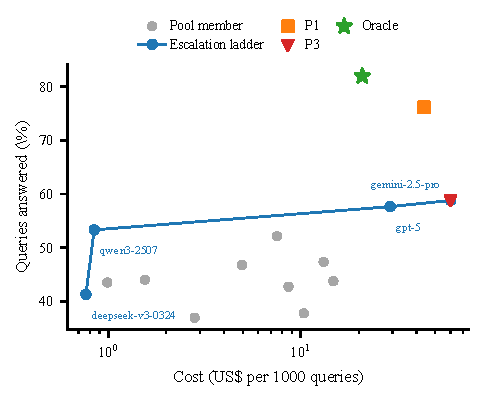
\includegraphics[width=\columnwidth]{figures/public_frontier}}
\caption{The thirteen models of the public pool, the cost--accuracy
frontier they define and where the escalation policies land on it. Cost is
logarithmic, in US dollars per 1{,}000 queries. P3 sits on the top rung it
always uses. P1 climbs the frontier and answers more queries than any
single model in the pool, at a price between the two costliest rungs. The
oracle answers still more for a third of what P3 costs.}
\label{fig:public-frontier}
\end{figure}

\begin{table*}[!t]
\caption{The public pool in cost order, over the 12{,}168 queries of nine
datasets that all thirteen models answered. Cost is the provider's own
charge, in US dollars per 1{,}000 queries. The $c^*$ share is the fraction
of queries for which that model is the cheapest one that answers
correctly, and the last row the queries no model answers. A bullet marks
the four models on the cost--accuracy frontier, which are the rungs of the
escalation ladder.}
\label{tab:public-pool}
\centering
\generated{tables/public_pool.tex}{\setlength{\tabcolsep}{4pt}
\begin{tabular}{@{}lrrrrc@{}}
\toprule
Model & Acc.\ (\%) & Cost (\$/1{,}000) & \$ per solved (/1{,}000) & $c^*$ share (\%) & Ladder \\
\midrule
\texttt{deepseek-v3-0324} & 41.3 & 0.76 & 1.85 & 7.1 & $\bullet$ \\
\texttt{qwen3-235b-a22b-2507} & 53.3 & 0.84 & 1.58 & 39.4 & $\bullet$ \\
\texttt{deepseek-v3.1-terminus} & 43.5 & 0.99 & 2.27 & 9.6 &  \\
\texttt{kimi-k2-0905} & 44.0 & 1.55 & 3.52 & 4.0 &  \\
\texttt{intern-s1} & 36.9 & 2.81 & 7.61 & 1.9 &  \\
\texttt{gpt-5-chat} & 46.8 & 4.95 & 10.59 & 3.4 &  \\
\texttt{qwen3-235b-a22b-thinking-2507} & 52.1 & 7.52 & 14.43 & 1.5 &  \\
\texttt{gemini-2.5-flash} & 42.7 & 8.63 & 20.23 & 5.7 &  \\
\texttt{claude-sonnet-4} & 37.7 & 10.36 & 27.47 & 0.5 &  \\
\texttt{deepseek-r1-0528} & 47.3 & 13.14 & 27.77 & 1.5 &  \\
\texttt{glm-4.6} & 43.7 & 14.78 & 33.78 & 1.6 &  \\
\texttt{gpt-5} & 57.6 & 29.15 & 50.57 & 3.4 & $\bullet$ \\
\texttt{gemini-2.5-pro} & 58.8 & 60.02 & 102.08 & 2.4 & $\bullet$ \\
\midrule
No model answers & -- & -- & -- & 18.0 &  \\
\bottomrule
\end{tabular}
}
\end{table*}

\begin{table*}[!t]
\caption{Escalation policies on the public pool under oracle detection, in
US dollars per 1{,}000 queries. P1 climbs the cost--accuracy frontier, P3
uses its top rung once, P4 starts uniformly over the pool and then climbs,
and Random picks a model uniformly and recovers at the top rung. A policy
that answers fewer queries can show a negative tax, underpaying by
failing, so the tax is read beside the solved column.}
\label{tab:public-tax}
\centering
\generated{tables/public_tax.tex}{\setlength{\tabcolsep}{4pt}
\begin{tabular}{@{}lrrrrr@{}}
\toprule
Policy & Solved (\%) & Attempts & Cost (\$/1{,}000) [95\% CI] & Tax [95\% CI] & Tax / $c^*$ cost \\
\midrule
P1, climb the frontier & 76.2 & 2.27 & 43.73 [41.98, 45.54] & 16.12 [15.11, 17.17] & 2.69 \\
P3, sticky top & 58.8 & 1.00 & 60.02 [58.62, 61.41] & 47.74 [46.41, 49.04] & 7.96 \\
P4, uniform start & 71.0 & 1.83 & 54.03 [52.34, 55.77] & 28.28 [27.25, 29.29] & 4.72 \\
Random, then top & 64.5 & 1.50 & 47.22 [45.82, 48.61] & 29.48 [28.44, 30.51] & 4.92 \\
\midrule
Always \texttt{deepseek-v3-0324} & 41.3 & 1.00 & 0.76 [0.74, 0.79] & -5.31 [-5.86, -4.78] & -0.89 \\
Always \texttt{qwen3-235b-a22b-2507} & 53.3 & 1.00 & 0.84 [0.81, 0.87] & -5.27 [-5.82, -4.75] & -0.88 \\
Always \texttt{gpt-5} & 57.6 & 1.00 & 29.15 [28.31, 30.01] & 18.34 [17.69, 19.01] & 3.06 \\
Always \texttt{gemini-2.5-pro} & 58.8 & 1.00 & 60.02 [58.62, 61.41] & 47.74 [46.41, 49.04] & 7.96 \\
\midrule
Oracle & 82.0 & 1.00 & 20.88 [19.84, 21.96] & 0.00 [0.00, 0.00] & 0.00 \\
\bottomrule
\end{tabular}
}
\end{table*}

The local grid stops at 8B parameters. Section~\ref{sec:public-arm}
recomputes the same quantities on the published outcomes of
LLMRouterBench: thirteen flagship models, nine datasets and 12{,}168
queries every model answered, priced by the providers themselves.

Table~\ref{tab:public-pool} and Fig.~\ref{fig:public-frontier} give the
pool in cost order. Its members span
a factor of 79 in price, from \$0.76 to \$60.02 per thousand queries, and
a factor of 1.6 in accuracy, from 36.9\% to 58.8\%. Price and accuracy are
only loosely related: of the eleven models dearer than
\texttt{qwen3-235b-a22b-2507}, nine answer fewer queries than it does. Only
four of the thirteen lie on the cost--accuracy frontier, and those four
are the ladder a rational escalator would climb. Between them the thirteen
answer 82.0\% of the queries; the remaining 18.0\% are beyond the pool.
The distribution of the minimum sufficient model repeats what the local
grid shows: the two cheapest models are the cheapest sufficient choice for
46.5\% of all queries, and the costliest model is that choice for 2.4\%.
Another 29.8\% are answered most cheaply by a model off the frontier,
which matters for what follows.

Table~\ref{tab:public-tax} gives the policies. Sticky use of the top of
the ladder (P3) costs 7.96 times the minimum sufficient cost, close to the
local grid's figure, and answers 58.8\% of queries. Climbing the frontier
(P1) costs 2.69 times, answers 76.2\% and takes 2.27 attempts per query.
The oracle answers 82.0\% at \$20.88 per thousand queries. Per solved
query the ordering is the same and the comparison is fair across policies
of unequal success: \$25.47 for the oracle, \$57.38 for P1 and \$102.08
for P3, so a user who always reaches for the strongest model pays four
times what a perfect one-shot router would pay for the same answers.

Two features of the pool are worth separating from the local grid. First,
the frontier is a subset: a policy climbing it fails on queries only an
off-frontier model answers, and then pays four cheap attempts instead of
one expensive sufficient model. This is why the two cheapest static
policies show a negative tax, and why on SimpleQA even P1 does; they
underpay by failing, answering 41.3\% and 53.3\% of queries. Tax is
meaningful only beside the success rate, which is why cost per solved
query carries the comparison. Second, the dollar tax is larger than the
token tax --- 7.96 against 2.04 for P3 --- because the price per token
spans two orders of magnitude across providers while the answers
themselves do not differ in length nearly as much. Escalation on a mixed
pool is expensive in a way that token counts hide.

The thinking and non-thinking releases of Qwen3-235B-A22B give the public
counterpart of the mode axis. Thinking costs 9.11 times more per solved
query [8.78, 9.47] and, over all nine datasets, answers slightly fewer
queries (52.1\% against 53.3\%). The plain release already answers 53.3\%
of queries on its own and only 9.3\% need thinking, so the mode is worth
paying for on a small minority of queries and is picked per query or not
at all. Where reasoning is the point the picture reverses --- on GPQA
thinking answers 80.3\% against 58.6\% --- which is the same
family-dependence the local grid shows.

Scoring a judged Arena-Hard tie as half credit rather than requiring a
full score moves nothing: P3 pays 8.14 times the minimum sufficient cost
and P1 2.64 times, against 7.96 and 2.69.

\subsection{The Escalation Tax on a Hosted Frontier Ladder}
\label{sec:results-hosted}

\begin{figure}[!t]
\centering
\generated{figures/hosted_frontier.pdf}
{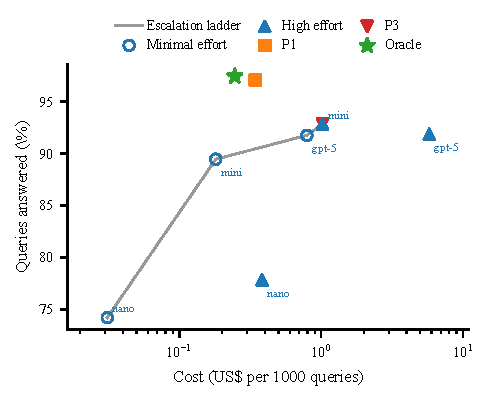
\includegraphics[width=\columnwidth]{figures/hosted_frontier}}
\caption{The six hosted cells on the cost--accuracy plane, open for
minimal reasoning effort and filled for high. Cost is logarithmic, in US
dollars per 1{,}000 queries. The grey line is the frontier the escalation
policies climb. The mode axis reads as the horizontal step from an open
marker to the filled marker of the same model.}
\label{fig:hosted-frontier}
\end{figure}

\begin{table*}[!t]
\caption{The six hosted cells: three model sizes crossed with two
reasoning efforts, on the prompts of the local main subset. Output tokens
include reasoning tokens, which the provider reports separately but bills
as output. A cap hit is a truncated generation, counted as a failure
exactly as a local cap hit is.}
\label{tab:hosted-cells}
\centering
\generated{tables/hosted_cells.tex}{\setlength{\tabcolsep}{3pt}
\begin{tabular}{@{}lllrrrrrr@{}}
\toprule
Cell & Model & Effort & Cap & Acc.\ (\%) & Out.\ tok. & Reas.\ tok. & Cap hit (\%) & Cost (\$/1{,}000) \\
\midrule
$h_1$ & \texttt{gpt-5-nano} & Minimal & 2{,}048 & 62.5 & 108 & 0 & 0.0 & 0.02 \\
$h_2$ & \texttt{gpt-5-nano} & High & 4{,}096 & 85.0 & 1{,}738 & 1{,}664 & 12.5 & 0.35 \\
$h_3$ & \texttt{gpt-5-mini} & Minimal & 2{,}048 & 97.5 & 147 & 0 & 0.0 & 0.16 \\
$h_4$ & \texttt{gpt-5-mini} & High & 4{,}096 & 97.5 & 824 & 675 & 0.0 & 0.84 \\
$h_5$ & \texttt{gpt-5} & Minimal & 2{,}048 & 100.0 & 132 & 0 & 0.0 & 0.73 \\
$h_6$ & \texttt{gpt-5} & High & 4{,}096 & 100.0 & 887 & 760 & 0.0 & 4.50 \\
\bottomrule
\end{tabular}
}
\end{table*}

\begin{table*}[!t]
\caption{Escalation policies on the hosted ladder under oracle detection,
in US dollars per 1{,}000 queries. The static rows are the ladder rungs
used alone. As on the public pool, a policy that answers fewer queries can
show a negative tax by underpaying through failure, so the tax is read
beside the solved column.}
\label{tab:hosted-tax}
\centering
\generated{tables/hosted_tax.tex}{\setlength{\tabcolsep}{4pt}
\begin{tabular}{@{}lrrrrr@{}}
\toprule
Policy & Solved (\%) & Attempts & Cost (\$/1{,}000) [95\% CI] & Tax [95\% CI] & Tax / $c^*$ cost \\
\midrule
P1, climb the frontier & 100.0 & 1.40 & 0.08 [0.05, 0.14] & 0.02 [0.00, 0.06] & 0.34 \\
P3, sticky top & 100.0 & 1.00 & 0.73 [0.57, 0.90] & 0.66 [0.51, 0.83] & 10.60 \\
P4, uniform start & 99.6 & 1.10 & 1.15 [0.85, 1.49] & 1.09 [0.79, 1.42] & 17.41 \\
Random, then top & 100.0 & 1.10 & 1.18 [0.87, 1.51] & 1.11 [0.82, 1.44] & 17.81 \\
\midrule
Always $h_{1}$ & 62.5 & 1.00 & 0.02 [0.02, 0.03] & -0.04 [-0.06, -0.02] & -0.61 \\
Always $h_{3}$ & 97.5 & 1.00 & 0.16 [0.12, 0.21] & 0.10 [0.06, 0.14] & 1.57 \\
Always $h_{5}$ & 100.0 & 1.00 & 0.73 [0.57, 0.90] & 0.66 [0.51, 0.83] & 10.60 \\
\midrule
Oracle & 100.0 & 1.00 & 0.06 [0.05, 0.08] & 0.00 [0.00, 0.00] & 0.00 \\
\bottomrule
\end{tabular}
}
\end{table*}

\tbd{Written when the hosted main stage finishes: the ladder and where
high effort falls off it, the $c^*$ distribution against the local
grid's, the policy taxes, and the reasoning-token cost of the mode axis.}

\subsection{Carbon of the Escalation Tax}
\label{sec:results-carbon}

\begin{table}[!t]
\caption{Carbon of the escalation tax under oracle detection, in grams of
CO$_2$e per 1{,}000 queries. The kWh column is the policy's own energy for
those queries; every carbon figure follows from it by multiplication. The
four columns are grid carbon intensities in gCO$_2$e/kWh: 50 for a grid
carried by nuclear or hydro, 250 for a large renewable share, 475 for the
figure usually quoted as the global average, and 700 for a grid carried by
coal. They are round values spanning the range grids occupy, not
measurements of a named region.}
\label{tab:carbon}
\centering
\generated{tables/carbon.tex}{\begin{tabular}{@{}lrrrrr@{}}
\toprule
Policy & kWh & 50 & 250 & 475 & 700 \\
\midrule
P1, frugal climb & 0.242 & 2.35 & 11.76 & 22.35 & 32.93 \\
P2, think first & 0.719 & 22.94 & 114.70 & 217.93 & 321.16 \\
P3, sticky high & 0.800 & 34.31 & 171.57 & 325.99 & 480.40 \\
P4, uniform start & 0.438 & 12.71 & 63.55 & 120.74 & 177.94 \\
P4, start skewed to $c_8$ & 0.593 & 21.97 & 109.84 & 208.71 & 307.57 \\
Random, then $c_8$ & 0.585 & 21.60 & 108.01 & 205.22 & 302.43 \\
Oracle & 0.164 & 0.00 & 0.00 & 0.00 & 0.00 \\
\bottomrule
\end{tabular}
}
\end{table}

\tbd{Written with the local energy results: the tax in carbon terms, and
whether the bracket is wide enough to reorder the policies.}
